% =====================================================================
%  MCMP117 -- Fundamentals of Operating Systems
%  Week 11 Course Notes: Permissions, Ownership & Users
%  Compile with XeLaTeX (twice):  xelatex MCMP117_Week11_Notes.tex
%  Needs ./figures/ and the ../code/ folder.
% =====================================================================
\documentclass[11pt,a4paper]{article}
\newcommand{\weeknum}{11}
% ---------- Page & fonts ---------------------------------------------
\usepackage[a4paper,margin=2.3cm,headheight=15pt]{geometry}
\usepackage{fontspec}
\IfFontExistsTF{Calibri}{\setmainfont{Calibri}}{\setmainfont{Carlito}}
\IfFontExistsTF{Cambria}{\newfontfamily\headfont{Cambria}}{\newfontfamily\headfont{Caladea}}
\IfFontExistsTF{Consolas}{\setmonofont[Scale=0.95]{Consolas}}{\setmonofont[Scale=0.88]{DejaVu Sans Mono}}
\usepackage{amsmath,amssymb}
\usepackage{microtype}
\linespread{1.12}
\setlength{\parskip}{0.55em}
\setlength{\parindent}{0pt}

% ---------- Colours (course design system) ----------------------------
\usepackage{xcolor}
\definecolor{dark}{HTML}{212121}
\definecolor{charcoal}{HTML}{36454F}
\definecolor{slate}{HTML}{50808E}
\definecolor{mint}{HTML}{02C39A}
\definecolor{mintdeep}{HTML}{028090}
\definecolor{light}{HTML}{F2F2F2}
\definecolor{muted}{HTML}{6B7679}

% ---------- Packages ---------------------------------------------------
\usepackage{graphicx}
\usepackage{float}
\usepackage{needspace}
\graphicspath{{figures/}}
\usepackage[font=small,labelfont={bf,color=mintdeep},justification=centering]{caption}
\usepackage{booktabs,longtable,array,tabularx}
\usepackage{enumitem}
\setlist{itemsep=0.25em,topsep=0.3em}
\usepackage{tikz}
\usetikzlibrary{arrows.meta,positioning,calc,shapes.geometric}
\usepackage{pgfplots}
\pgfplotsset{compat=1.17}
\usepackage[most]{tcolorbox}
\usepackage{titlesec}
\usepackage{fancyhdr}
\usepackage{xurl}
\usepackage[colorlinks=true,linkcolor=mintdeep,urlcolor=mintdeep,citecolor=mintdeep]{hyperref}

% ---------- Headings ----------------------------------------------------
\titleformat{\section}{\headfont\Large\bfseries\color{charcoal}}{\color{mint}\thesection}{0.7em}{}
\titleformat{\subsection}{\headfont\large\bfseries\color{charcoal}}{\color{mintdeep}\thesubsection}{0.6em}{}
\titleformat{\subsubsection}{\headfont\normalsize\bfseries\color{mintdeep}}{}{0em}{}
\titlespacing*{\section}{0pt}{1.6em}{0.6em}
\titlespacing*{\subsection}{0pt}{1.2em}{0.4em}

% ---------- Header / footer -----------------------------------------------
\pagestyle{fancy}
\fancyhf{}
\fancyhead[L]{\small\color{muted}MCMP117 --- Fundamentals of Operating Systems}
\fancyhead[R]{\small\color{muted}Week \weeknum{} Notes}
\fancyfoot[C]{\small\color{muted}\thepage}
\renewcommand{\headrulewidth}{0pt}

% ---------- Boxes ---------------------------------------------------------
\newtcolorbox{keyidea}[1][Key idea]{enhanced,breakable,colback=charcoal,colframe=charcoal,
  coltext=white,fonttitle=\headfont\bfseries\color{mint},title={#1},
  attach title to upper={\par\smallskip},boxrule=0pt,arc=3pt,left=10pt,right=10pt,top=8pt,bottom=8pt}
\newtcolorbox{example}[1][Worked example]{enhanced,colback=light,colframe=light,
  fonttitle=\headfont\bfseries\color{mintdeep},title={#1},attach title to upper={\par\smallskip},
  boxrule=0pt,arc=3pt,left=10pt,right=10pt,top=8pt,bottom=8pt}
\newtcolorbox{tryit}[1][Try it yourself]{enhanced,breakable,colback=white,colframe=mint,
  fonttitle=\headfont\bfseries\color{mintdeep},title={#1},attach title to upper={\par\smallskip},
  boxrule=0.8pt,arc=3pt,left=10pt,right=10pt,top=8pt,bottom=8pt}
\newtcolorbox{histnote}[1][Historical note]{enhanced,breakable,colback=white,colframe=slate!40,
  fonttitle=\headfont\bfseries\color{slate},title={#1},attach title to upper={\par\smallskip},
  boxrule=0.5pt,arc=3pt,left=10pt,right=10pt,top=8pt,bottom=8pt,fontupper=\small}

% Photo helper: fits image inside a box, never distorted (keepaspectratio)
\newcommand{\photo}[3]{\includegraphics[width=#1,height=#2,keepaspectratio]{#3}}

\newcommand{\term}[1]{\textbf{\color{mintdeep}#1}}
\newcommand{\cmd}[1]{\texttt{#1}}


% ---------- Code listings ----------------------------------------------------
\usepackage{listings}
\lstdefinestyle{course}{
  basicstyle=\ttfamily\small, columns=fullflexible, keepspaces=true,
  backgroundcolor=\color{dark}, rulecolor=\color{dark}, frame=single, framesep=6pt,
  xleftmargin=8pt, xrightmargin=8pt, aboveskip=0.8em, belowskip=0.6em,
  basicstyle=\ttfamily\small\color{light},
  keywordstyle=\color{mint}\bfseries, commentstyle=\color{white!60}\itshape,
  stringstyle=\color{orange!70!yellow}, numberstyle=\tiny\color{muted},
  numbers=left, numbersep=10pt, showstringspaces=false, breaklines=true,
  tabsize=4, upquote=true}
\lstdefinestyle{term}{style=course, numbers=none, keywordstyle=\color{light},
  commentstyle=\color{white!60}, stringstyle=\color{light}}
\lstset{style=course,language=C}
\usepackage{textcomp}

\begin{document}
% ============================ Week 11 body ============================
% terminal transcripts in this week are long: print them one size smaller
\lstdefinestyle{term}{style=course, numbers=none, keywordstyle=\color{light},
  commentstyle=\color{white!60}, stringstyle=\color{light}, basicstyle=\ttfamily\footnotesize\color{light}}
\thispagestyle{empty}
\begin{tcolorbox}[enhanced,colback=dark,colframe=dark,arc=0pt,boxrule=0pt,
  left=18pt,right=18pt,top=20pt,bottom=20pt,coltext=white]
{\small\color{mint}\textsc{MCMP117 \,·\, Week 11 \,·\, Course Notes}}\par\medskip
{\headfont\fontsize{26}{30}\selectfont\bfseries Fundamentals of Operating Systems}\par\medskip
{\large Permissions, Ownership \& Users}\par\smallskip
{\small\itshape\color{white!70} Who may read, change or run your files --- and how does Linux decide?}
\end{tcolorbox}

\vspace{0.4em}
{\small
\textbf{Instructor:} Asst.\ Prof.\ Dr.\ (Ph.D.) Hasan Oğuz\\
Head of the Electronical Communication Technology Programme, Vocational School\\
Istanbul Okan University\par}

\vspace{0.8em}
\begin{keyidea}[What you should be able to do after this week]
\begin{enumerate}[leftmargin=1.4em]
  \item Explain why an operating system needs file permissions and how the kernel enforces them (links to Week~2 and Week~7).
  \item Find your user name, UID, GID and groups with \cmd{whoami}, \cmd{id} and \cmd{groups}, and read the fields of \texttt{/etc/passwd} and \texttt{/etc/group}.
  \item Decode a mode string such as \texttt{-rwxr-x---} and convert it to octal ($750$) and back.
  \item Explain what $r$, $w$ and $x$ mean for files \emph{and} for directories, and which of owner, group and others applies to a process.
  \item Change permissions with \cmd{chmod} in symbolic (\texttt{u+x}, \texttt{go-w}) and octal (\texttt{640}) form, and make a script executable.
  \item Compute default permissions from the \cmd{umask} correctly (bitwise, not by subtraction).
  \item Explain \cmd{chown}, \cmd{chgrp}, \cmd{sudo}, the setuid bit of \cmd{passwd} and the sticky bit of \texttt{/tmp}, and read the related error messages.
\end{enumerate}
\end{keyidea}

\setcounter{tocdepth}{1}
\tableofcontents

% =====================================================================
\section{From Week 10 to Week 11}

Last week you created, copied, moved and deleted files (\cmd{mkdir}, \cmd{touch}, \cmd{cp}, \cmd{mv}, \cmd{rm}), let the shell expand wildcards, and looked at files with \cmd{cat}, \cmd{less}, \cmd{head}, \cmd{tail} and \cmd{stat}. Every \cmd{ls -l} and \cmd{stat} printed something like \texttt{-rw-rw-r--} and \texttt{Access: (0664/-rw-rw-r--)}, together with the names of an owner and a group. This week we learn to read these fields, to change them, and to understand the users and groups behind them.

\paragraph{How to follow the examples.} Re-create the practice folder first (it deletes and re-creates only \texttt{\textasciitilde/lab}):
\begin{lstlisting}[style=term]
$ bash mcmp117_lab_setup.sh
\end{lstlisting}
Every command in these notes was run on a Linux machine as an \emph{ordinary} user called \texttt{student} (host \texttt{okan-lab}); the scripts \texttt{code/demo\_*.sh} contain the exact commands and \texttt{code/out\_*.txt} the captured output. On your machine dates, sizes, user and group \emph{numbers} and names will differ, and the order of \cmd{ls} output can depend on the locale (we used \texttt{LC\_ALL=C.UTF-8}). Only where the topic is \cmd{sudo} or \texttt{root} do we say explicitly that an administrator prepared something.

% =====================================================================
\section{Why Permissions? Protection Revisited}

\subsection{The theory behind it}

In \textbf{Week~2} we saw \term{dual-mode operation}: the CPU runs user programs in \emph{user mode}, where privileged instructions such as direct I/O are forbidden. A program that wants to read a file cannot talk to the disk itself; it must make a \term{system call} such as \cmd{open()}, which switches to kernel mode. In \textbf{Week~7} we listed \emph{protection} as one of the attributes of a file and saw that Linux stores it in the file's \term{inode}, together with the owner, the group, the size and the timestamps.

Put these two facts together and you have the whole mechanism:

\begin{figure}[H]
\centering
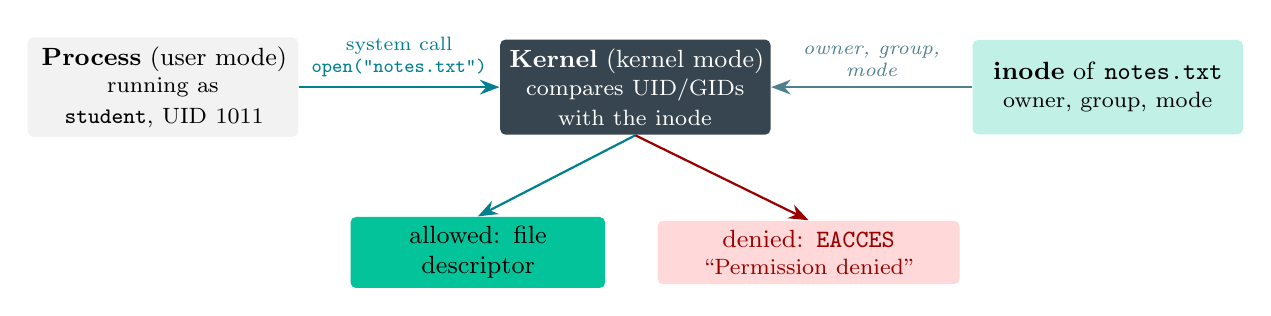
\begin{tikzpicture}[b/.style={rectangle,rounded corners=2pt,minimum height=1.2cm,align=center,font=\small,text width=3.2cm},
  arr/.style={-{Stealth[length=2.5mm]},thick}]
\node[b,fill=light] (p) at (0,0) {\textbf{Process} (user mode)\\[-1pt]{\footnotesize running as \texttt{student}, UID 1011}};
\node[b,fill=charcoal,text=white] (k) at (6.0,0) {\textbf{Kernel} (kernel mode)\\[-1pt]{\footnotesize compares UID/GIDs with the inode}};
\node[b,fill=mint!25] (i) at (12.0,0) {\textbf{inode} of \texttt{notes.txt}\\[-1pt]{\footnotesize owner, group, mode}};
\draw[arr,mintdeep] (p) -- node[above,font=\scriptsize,align=center]{system call\\\texttt{open("notes.txt")}} (k);
\draw[arr,slate] (i) -- node[above,font=\scriptsize\itshape,align=center]{owner, group,\\mode} (k);
\node[b,fill=mint,text width=3.0cm,minimum height=0.8cm] (ok) at (4.0,-2.1) {allowed: file descriptor};
\node[b,fill=red!15,text=red!60!black,text width=3.6cm,minimum height=0.8cm] (no) at (8.2,-2.1) {denied: \texttt{EACCES}\\[-1pt]{\footnotesize ``Permission denied''}};
\draw[arr,mintdeep] (k.south) -- (ok.north);
\draw[arr,red!60!black] (k.south) -- (no.north);
\end{tikzpicture}
\caption{Every access goes through a system call, so the kernel can check it and it cannot be skipped.}
\end{figure}

Because the program \emph{has} to ask the kernel, the kernel can refuse. If the check fails, the system call returns $-1$ and sets the error code \texttt{EACCES}; programs print it as \emph{Permission denied}. The same check happens when you run a program (\cmd{exec}), enter a directory (\cmd{chdir}) or delete a name (\cmd{unlink}). Note that the check is made when the file is \emph{opened}: a process that already has a file open keeps its access even if the permissions change afterwards.


\begin{histnote}
UNIX, designed at Bell Labs from 1969, was a multi-user time-sharing system from the start (Week~1), so it needed a cheap protection scheme. Instead of a full list of users per file (an \emph{access control list}), Ken Thompson and Dennis Ritchie chose three classes --- owner, group, others --- with three bits each: nine bits in the inode. The scheme was so simple and effective that it survives unchanged in Linux and macOS. (Modern Linux also supports ACLs with \cmd{getfacl}/\cmd{setfacl}, but the nine bits remain the basis.)
\end{histnote}

% =====================================================================
\section{Users and Groups}

\subsection{Who am I?}
\label{sec:who}

Linux knows two kinds of identity:
\begin{itemize}
  \item A \term{user} has a login name and a number, the \term{UID} (user ID). The kernel stores and compares only the number. The user \texttt{root} has UID $0$ and is the \term{superuser}. Many \emph{system users} (for example \texttt{daemon} or \texttt{www-data}) exist only to run services with limited rights.
  \item A \term{group} is a named set of users with a number, the \term{GID}. Each user has exactly one \emph{primary group} and may belong to several \emph{supplementary groups}. Ubuntu creates a private group with the same name for every user.
\end{itemize}
Every process carries the UID and GIDs of the user who started it (its \emph{credentials}); a file it creates gets that UID as owner and the primary GID as group.

\lstinputlisting[style=term,firstline=1,lastline=6]{../code/out_users.txt}

Here \texttt{uid=1011(student)} is the user number and name, \texttt{gid=1013(student)} the primary group, and \texttt{groups=} lists every group. On a freshly installed Ubuntu the first user normally has UID $1000$; our lab machine has more accounts.

\subsection{The account files \texttt{/etc/passwd} and \texttt{/etc/group}}

\lstinputlisting[style=term,firstline=7,lastline=20]{../code/out_users.txt}

A line of \texttt{/etc/passwd} has seven fields separated by colons:

\begin{figure}[H]
\centering
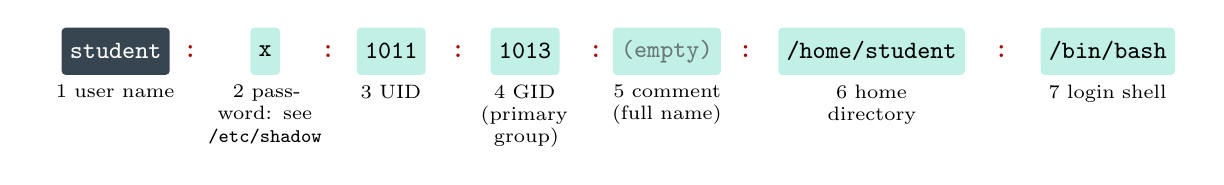
\begin{tikzpicture}[f/.style={rectangle,rounded corners=1.5pt,fill=mint!25,minimum height=0.6cm,font=\ttfamily\small,inner sep=3pt},
  l/.style={font=\scriptsize,align=center,text width=2.0cm,anchor=north}]
\node[f,fill=charcoal,text=white] (a) at (0,0) {student};
\node[f] (b) at (1.9,0) {x};
\node[f] (c) at (3.5,0) {1011};
\node[f] (d) at (5.2,0) {1013};
\node[f,text=muted] (e) at (7.0,0) {(empty)};
\node[f] (g) at (9.6,0) {/home/student};
\node[f] (h) at (12.6,0) {/bin/bash};
\foreach \x in {0.95,2.7,4.35,6.1,8.0,11.25} \node[font=\bfseries\ttfamily,text=red!70!black] at (\x,0) {:};
\node[l] at (a.south) {1 user name};
\node[l,text width=1.6cm] at (b.south) {2 password: see \texttt{/etc/shadow}};
\node[l,text width=1.2cm] at (c.south) {3 UID};
\node[l,text width=1.3cm] at (d.south) {4 GID (primary group)};
\node[l,text width=1.5cm] at (e.south) {5 comment (full name)};
\node[l] at (g.south) {6 home directory};
\node[l] at (h.south) {7 login shell};
\end{tikzpicture}
\caption{The seven fields of a line of \texttt{/etc/passwd}.}
\end{figure}

A line of \texttt{/etc/group} has four fields: group name, password (unused, \texttt{x}), GID and a comma-separated list of members. The group \texttt{students} has no members yet (empty fourth field).

Why is the password not in \texttt{/etc/passwd}? Every program must be able to \emph{read} \texttt{/etc/passwd} --- \cmd{ls} needs it to turn UIDs into names. The password \emph{hashes} are therefore kept in \texttt{/etc/shadow}, whose mode \texttt{-rw-r-----} lets only \texttt{root} and the group \texttt{shadow} read it. That is why \cmd{cat /etc/shadow} fails for us. Administrators never edit these files by hand; they use \cmd{useradd}, \cmd{usermod}, \cmd{groupadd} and \cmd{passwd}.

% =====================================================================
\section{Reading Permissions}

\subsection{The columns of \cmd{ls -l}}

\lstinputlisting[style=term,firstline=12,lastline=21]{../code/out_ls.txt}

The columns are: (1) file type and permissions, (2) link count (Week~7, Week~10), (3) owner, (4) group, (5) size in bytes, (6) modification time and (7) the name. Everything except the name comes from the inode; the name comes from the directory entry. The inode stores \emph{numbers} for owner and group; \cmd{ls} shows names by looking them up in \texttt{/etc/passwd} and \texttt{/etc/group}. Note the difference between \cmd{ls -l docs} (the files \emph{inside} \texttt{docs}) and \cmd{ls -ld docs} (the directory itself).

\subsection{Decoding the mode string}

\begin{figure}[H]
\centering
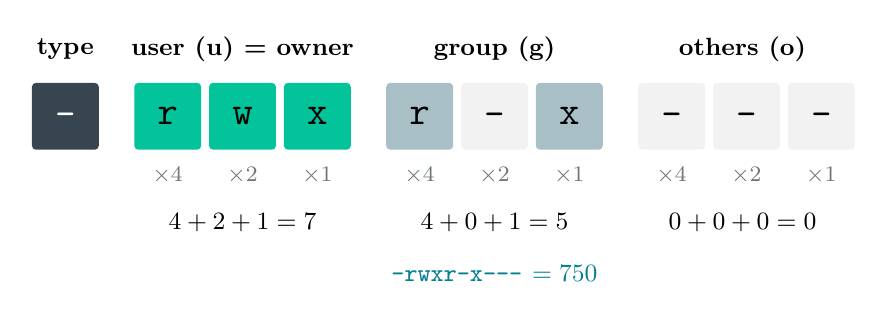
\begin{tikzpicture}[bt/.style={rectangle,rounded corners=1.5pt,minimum width=0.85cm,minimum height=0.85cm,font=\ttfamily\Large\bfseries}]
\def\bw{0.95}
\node[bt,fill=charcoal,text=white] at (0,0) {-};
\foreach \i/\c/\col in {0/r/mint,1/w/mint,2/x/mint,3/r/slate!50,4/-/light,5/x/slate!50,6/-/light,7/-/light,8/-/light} {
  \pgfmathsetmacro{\xx}{1.3+\i*\bw+floor(\i/3)*0.35}
  \node[bt,fill=\col] at (\xx,0) {\c};
  \pgfmathsetmacro{\w}{int(mod(\i,3)==0 ? 4 : (mod(\i,3)==1 ? 2 : 1))}
  \node[font=\footnotesize,text=muted] at (\xx,-0.75) {$\times\w$};
}
\node[font=\small\bfseries] at (0,0.85) {type};
\node[font=\small\bfseries] at (2.25,0.85) {user (u) = owner};
\node[font=\small\bfseries] at (5.45,0.85) {group (g)};
\node[font=\small\bfseries] at (8.6,0.85) {others (o)};
\node[font=\small] at (2.25,-1.35) {$4+2+1=7$};
\node[font=\small] at (5.45,-1.35) {$4+0+1=5$};
\node[font=\small] at (8.6,-1.35) {$0+0+0=0$};
\node[font=\small\bfseries,text=mintdeep] at (5.45,-2.0) {\texttt{-rwxr-x---} $= 750$};
\end{tikzpicture}
\caption{The first character is the type; then three triplets for user, group and others; each bit has weight $4$, $2$ or $1$.}
\label{fig:mode}
\end{figure}

\begin{itemize}
  \item \textbf{Character 1, the type:} \texttt{-} regular file, \texttt{d} directory, \texttt{l} symbolic link, \texttt{c}/\texttt{b} character/block device.
  \item \textbf{Characters 2--10:} three \emph{triplets}, always in the order user (the owner), group, others; inside each triplet always $r$, $w$, $x$. A letter means the permission is granted, a dash that it is not.
\end{itemize}
Each triplet has $3$ bits, so there are $2^3 = 8$ possible triplets --- exactly the eight octal digits $0$--$7$. With weights $r = 4$, $w = 2$, $x = 1$, every triplet is a single digit, and the nine bits are written as three octal digits: \texttt{-rwxr-x---} is $750$. The command \cmd{stat} shows both forms; \cmd{stat -c} lets you choose the fields:

\lstinputlisting[style=term,firstline=31,lastline=34]{../code/out_ls.txt}

\subsection{What r, w and x mean}

\begin{center}
\small
\begin{tabularx}{\linewidth}{@{}l X X@{}}
\toprule
\textbf{Bit} & \textbf{On a regular file} & \textbf{On a directory} \\
\midrule
$r$ ($4$) & read the contents (\cmd{cat}, \cmd{less}, \cmd{cp}) & list the names inside (\cmd{ls}) \\
$w$ ($2$) & change the contents (editor, \texttt{>>}) & create, delete and rename entries (together with $x$) \\
$x$ ($1$) & run it as a program or script & enter it and reach what is inside (\cmd{cd}, paths through it) \\
\bottomrule
\end{tabularx}
\end{center}

Remember from Week~7 that a directory is a table of (name, inode number) pairs. Reading the table means listing names; writing it means adding or removing entries; $x$ (``search'') means following a path through it. Two consequences surprise most beginners: deleting a file is a change to the \emph{directory}, so it needs $w$ on the directory and does not depend on the file's own $w$ bit; and without $x$ on a directory nothing below it can be reached, however generous the files' own permissions are. Section~\ref{sec:dirs} demonstrates both.

\subsection{Which class applies? Only one}

When a process accesses a file, the kernel does \emph{not} combine the three triplets. It picks exactly one:

\begin{figure}[H]
\centering
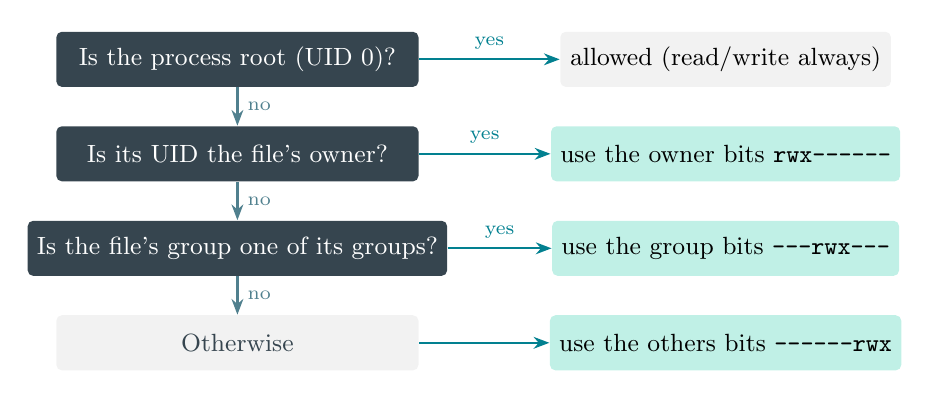
\begin{tikzpicture}[q/.style={rectangle,rounded corners=2pt,fill=charcoal,text=white,minimum width=4.6cm,minimum height=0.7cm,font=\small},
  a/.style={rectangle,rounded corners=2pt,fill=mint!25,minimum width=4.2cm,minimum height=0.7cm,font=\small},
  arr/.style={-{Stealth[length=2mm]},thick}]
\node[q] (q1) at (0,0) {Is the process root (UID 0)?};
\node[q] (q2) at (0,-1.2) {Is its UID the file's owner?};
\node[q] (q3) at (0,-2.4) {Is the file's group one of its groups?};
\node[q,fill=light,text=charcoal] (q4) at (0,-3.6) {Otherwise};
\node[a,fill=light] (a1) at (6.2,0) {allowed (read/write always)};
\node[a] (a2) at (6.2,-1.2) {use the owner bits \texttt{rwx------}};
\node[a] (a3) at (6.2,-2.4) {use the group bits \texttt{---rwx---}};
\node[a] (a4) at (6.2,-3.6) {use the others bits \texttt{------rwx}};
\foreach \i in {1,2,3} \draw[arr,mintdeep] (q\i) -- node[above,font=\scriptsize]{yes} (a\i);
\draw[arr,mintdeep] (q4) -- (a4);
\foreach \i/\j in {1/2,2/3,3/4} \draw[arr,slate] (q\i) -- node[right,font=\scriptsize]{no} (q\j);
\end{tikzpicture}
\caption{The kernel's access check stops at the first class that matches.}
\end{figure}

So the owner is judged \emph{only} by the owner triplet, even if the others triplet is more generous. Our demonstration (\cmd{code/demo\_order.sh}):

\lstinputlisting[style=term]{../code/out_order.txt}

With mode $074$ = \texttt{----rwxr--} everybody else may read, but the owner may not. The owner can still repair the situation, because changing the mode requires \emph{ownership}, not $r$ or $w$. (For \texttt{root}, read and write are always allowed; execute is allowed if at least one $x$ bit is set.)

% =====================================================================
\section{Changing Permissions with \cmd{chmod}}

Only the owner of a file (or \texttt{root}) may change its mode. \cmd{chmod} (\emph{change mode}) accepts two notations.

\subsection{Symbolic mode}

The form is \texttt{chmod} \emph{who operator permissions} \emph{file\dots}:
\begin{itemize}
  \item \textbf{who:} \texttt{u} (user = owner), \texttt{g} (group), \texttt{o} (others), \texttt{a} (all three);
  \item \textbf{operator:} \texttt{+} add, \texttt{-} remove, \texttt{=} set exactly (the unnamed bits of that class are cleared);
  \item \textbf{permissions:} any of \texttt{r}, \texttt{w}, \texttt{x}.
\end{itemize}
Several clauses are separated by commas \emph{without spaces}: \texttt{u=rw,g=r,o=} (the empty \texttt{o=} means ``no rights for others''). The session below (\cmd{code/demo\_chmod\_sym.sh}) changes \texttt{docs/syllabus.txt} step by step:

\lstinputlisting[style=term]{../code/out_chmod_sym.txt}

\cmd{chmod} prints nothing when it succeeds (``no news is good news''); always check with \cmd{ls -l} or \cmd{stat}. \texttt{+} and \texttt{-} leave the other bits untouched, which makes symbolic mode ideal for small changes such as ``also let the group write'' (\texttt{chmod g+w}). Writing \cmd{chmod +x file} without a class adds $x$ for every class \emph{not blocked by the umask} (Section~\ref{sec:umask}); \texttt{u+x} is clearer.

\subsection{Octal mode}

In octal mode you give all nine bits at once, one digit per class:

\begin{center}
\small
\begin{tabular}{@{}c c c l@{}}
\toprule
\textbf{Octal} & \textbf{Binary} $r\,w\,x$ & \textbf{Symbolic} & \textbf{Meaning} \\
\midrule
$0$ & $000$ & \texttt{---} & no access \\
$1$ & $001$ & \texttt{--x} & execute only \\
$2$ & $010$ & \texttt{-w-} & write only (rare) \\
$3$ & $011$ & \texttt{-wx} & write and execute (rare) \\
$4$ & $100$ & \texttt{r--} & read only \\
$5$ & $101$ & \texttt{r-x} & read and execute \\
$6$ & $110$ & \texttt{rw-} & read and write \\
$7$ & $111$ & \texttt{rwx} & everything \\
\bottomrule
\end{tabular}
\end{center}

Because $4$, $2$ and $1$ are powers of two, every digit from $0$ to $7$ is a \emph{unique} sum of them: this is simply binary, three bits at a time. Two quick checks: an odd digit always contains $x$; a digit $\ge 4$ always contains $r$.

\begin{example}[Converting in both directions]
\textbf{Symbolic $\to$ octal.} \texttt{rwxr-xr--}: $\texttt{rwx} = 4+2+1 = 7$, $\texttt{r-x} = 4+0+1 = 5$, $\texttt{r--} = 4+0+0 = 4$, so the mode is $754$. Likewise \texttt{rw-rw-r--} $= 664$ and \texttt{rw-r-----} $= 640$.

\textbf{Octal $\to$ symbolic.} $711$: $7 = 4+2+1 \to$ \texttt{rwx}, $1 \to$ \texttt{--x}, $1 \to$ \texttt{--x}, so \texttt{rwx--x--x}. $640$: $6 = 4+2 \to$ \texttt{rw-}, $4 \to$ \texttt{r--}, $0 \to$ \texttt{---}: \texttt{rw-r-----}.

(All conversions in these notes were checked with \cmd{code/perm\_check.py}.)
\end{example}

\begin{center}
\small
\begin{tabularx}{\linewidth}{@{}l l X@{}}
\toprule
\textbf{Octal} & \textbf{Symbolic} & \textbf{Typical use} \\
\midrule
$644$ & \texttt{rw-r--r--} & ordinary files: everyone reads, only the owner writes \\
$755$ & \texttt{rwxr-xr-x} & programs, scripts and directories that others may use \\
$600$ & \texttt{rw-------} & private files (passwords, SSH keys --- \cmd{ssh} refuses a key that others can read) \\
$700$ & \texttt{rwx------} & private directories (\texttt{\textasciitilde/.ssh}) \\
$640$ / $750$ & \texttt{rw-r-----} / \texttt{rwxr-x---} & shared with the group, hidden from others \\
$777$ & \texttt{rwxrwxrwx} & everyone may change or delete: almost never correct \\
\bottomrule
\end{tabularx}
\end{center}

\begin{keyidea}[Safety: never ``fix'' an error with \texttt{chmod 777}]
\texttt{chmod 777} (or worse, \texttt{chmod -R 777}) makes a Permission-denied message disappear by letting \emph{every} user and every compromised program on the machine change or replace the file. Find the one missing bit and add only that, e.g.\ \texttt{chmod u+x script.sh}. This is the \emph{principle of least privilege}.
\end{keyidea}

The octal session (\cmd{code/demo\_chmod\_oct.sh}) also shows two typical errors:

\lstinputlisting[style=term]{../code/out_chmod_oct.txt}

The digits $8$ and $9$ do not exist in octal, and \texttt{rw} is neither a number nor a valid symbolic clause (it lacks \emph{who} and an operator: \texttt{u+rw}). A recursive change \cmd{chmod -R} applies the same mode to files \emph{and} directories; \texttt{chmod -R 644 dir} would remove $x$ from every subdirectory and lock you out. With \texttt{-R} prefer symbolic mode that only removes rights (\texttt{chmod -R go-rwx dir}), or the capital \texttt{X}, which adds $x$ only to directories (and files that already have an $x$).

\subsection{Making a script executable}
\label{sec:script}

A newly created file is never executable (Section~\ref{sec:umask} explains why). The session \cmd{code/demo\_script.sh}:

\lstinputlisting[style=term]{../code/out_script.txt}

\begin{itemize}
  \item Typing \cmd{./hello.sh} asks the kernel to \emph{execute} the file (system call \cmd{execve}); this requires $x$. \cmd{bash hello.sh} executes \cmd{bash}, which only \emph{reads} the file --- $r$ is enough.
  \item \cmd{hello.sh} without \texttt{./} is ``command not found'': the shell looks for commands only in the directories listed in \texttt{PATH}, and the current directory is not among them (for security). This is not a permission problem.
  \item The first line \texttt{\#!/bin/bash} (the \emph{shebang}) tells the kernel which interpreter runs the script. Week~14 builds on this.
  \item \cmd{gcc} sets the $x$ bits itself: it creates the program with $777$, reduced by the umask $002$ to $775$.
\end{itemize}

% =====================================================================
\section{Default Permissions: the \cmd{umask}}
\label{sec:umask}

Why are new files $664$ and new directories $775$? A program that creates a file asks for a mode in its \cmd{open()} or \cmd{mkdir()} call: editors, \cmd{touch} and the shell ask for $666$ (\texttt{rw-rw-rw-}) for files and $777$ for directories. The kernel then \emph{removes} every bit that is set in the process's \term{umask} (user file-creation mask). The umask is a per-process setting inherited by child processes; it is set at login (on Ubuntu to $002$ for normal users, $022$ for root) and can be changed with the shell built-in \cmd{umask}.

\subsection{It clears bits; it does not subtract}

Formally,
\[
\text{new mode} = \text{requested mode} \;\mathbin{\text{AND}}\; (\text{NOT umask}),
\]
applied bit by bit. For the common umask $022$ this looks like subtraction, $666 - 022 = 644$:
\[
\begin{array}{lrl}
\text{requested} & 666 = & 110\;110\;110 \\
\text{umask}     & 022 = & 000\;010\;010 \\
\text{NOT umask} &       & 111\;101\;101 \\ \hline
\text{AND}       &       & 110\;100\;100 = 644 = \texttt{rw-r--r--}
\end{array}
\]

\begin{example}[Where subtraction goes wrong: umask $033$]
The umask $033$ means: take $w$ and $x$ away from group and others. For a \emph{file}:
\[
\begin{array}{lrl}
\text{requested} & 666 = & 110\;110\;110 \\
\text{NOT } 033  &       & 111\;100\;100 \\ \hline
\text{AND}       &       & 110\;100\;100 = 644 = \texttt{rw-r--r--}
\end{array}
\]
Plain subtraction would give $666 - 033 = 633 = \texttt{rw--wx-wx}$: write and execute without read, and $x$ bits on a file that never asked for them. Nonsense! In each digit, $6 - 3 = 3$ ``borrows'' an $x$ bit that was never set, while the bitwise operation simply leaves an absent bit absent: $6 \mathbin{\text{AND}} \text{NOT}\,3 = 110 \mathbin{\text{AND}} 100 = 100 = 4$.

For a \emph{directory}, $777$ has every bit set, so subtraction happens to agree: $777 - 033 = 744$. In general, subtraction is correct exactly when every bit of the umask is also set in the requested mode. For files ($666$, no $x$ bits) it therefore fails for every umask containing an $x$ bit, e.g.\ $027$: $666 - 027 = 637$ (wrong) versus the correct $640$; and $077$: $666 - 077 = 567$ (wrong) versus $600$.
\end{example}

\begin{center}
\small
\begin{tabular}{@{}c l l l@{}}
\toprule
\textbf{umask} & \textbf{new file} ($666$) & \textbf{new directory} ($777$) & \textbf{typical use} \\
\midrule
$002$ & $664$ \texttt{rw-rw-r--} & $775$ \texttt{rwxrwxr-x} & Ubuntu users (private groups) \\
$022$ & $644$ \texttt{rw-r--r--} & $755$ \texttt{rwxr-xr-x} & root, many servers \\
$027$ & $640$ \texttt{rw-r-----} & $750$ \texttt{rwxr-x---} & group reads, others nothing \\
$077$ & $600$ \texttt{rw-------} & $700$ \texttt{rwx------} & fully private \\
$033$ & $644$ \texttt{rw-r--r--} & $744$ \texttt{rwxr--r--} & the subtraction trap \\
\bottomrule
\end{tabular}
\end{center}

The real session (\cmd{code/demo\_umask.sh}) confirms every row:

\lstinputlisting[style=term]{../code/out_umask.txt}

\cmd{umask -S} prints the complement in symbolic form, i.e.\ what is \emph{allowed}. Because files are requested without $x$, no umask can ever make a new file executable: that always takes a \cmd{chmod}. The umask is a property of the shell process, which is why \cmd{umask} (like \cmd{cd}) is built into the shell. A change lasts until the shell exits; to make it permanent, add e.g.\ \texttt{umask 027} to \texttt{\textasciitilde/.bashrc}. Existing files are never affected.

% =====================================================================
\section{Directory Permissions in Practice}
\label{sec:dirs}

The session \cmd{code/demo\_dirperm.sh} creates a directory \texttt{box} with one file and removes bits from it:

\lstinputlisting[style=term,firstline=1,lastline=24]{../code/out_dirperm.txt}

\begin{itemize}
  \item \textbf{$r$ without $x$:} \cmd{ls} can read the list of names, but \cmd{ls -l} cannot look up the inodes through the directory --- hence the question marks --- and \cmd{cd} and \cmd{cat} fail.
  \item \textbf{$x$ without $r$:} the directory cannot be listed, but a file whose name you know can be opened. (A building where you have a key to every room but no list of the rooms.)
\end{itemize}
In practice, directories have $r$ and $x$ together: \texttt{r-x} or \texttt{rwx}.

\lstinputlisting[style=term,firstline=25,lastline=38]{../code/out_dirperm.txt}

The file is read-only ($444$), so appending fails --- but \cmd{rm} merely asks a question and then deletes it, because deletion changes the \emph{directory} \texttt{box}, which is writable. Only when the directory itself becomes $555$ can nothing be added or removed.

\begin{keyidea}[Safety: \texttt{rm} and read-only files]
A read-only file is \emph{not} protected against deletion. \texttt{rm -f} even skips the question, and \texttt{rm -r} deletes whole trees without a recycle bin (Week~10). To protect files from deletion, remove $w$ from the directory that contains them.
\end{keyidea}

% =====================================================================
\section{Ownership: \cmd{chown} and \cmd{chgrp}}
\label{sec:own}

\cmd{chown user file} changes the owner (\cmd{chown user:group file} both); \cmd{chgrp group file} changes the group; both accept \texttt{-R}. The rules on Linux:
\begin{itemize}
  \item Only \texttt{root} may change the owner. Otherwise a user could ``give away'' files to escape a disk quota or make a file appear to be someone else's.
  \item The owner may change the group, but only to a group he or she belongs to.
\end{itemize}

\lstinputlisting[style=term]{../code/out_owner.txt}

Note the different message: \emph{Operation not permitted} (\texttt{EPERM}) means that the operation needs a privilege, whatever the permission bits; \emph{Permission denied} (\texttt{EACCES}) means a permission bit is missing.

\subsection{Sharing a folder with a group}

For the next session the administrator ran \cmd{sudo usermod -aG students student} (add, \texttt{-a}, to the supplementary group, \texttt{-G}, \texttt{students}) and the student logged in again --- group membership is read at login. (Without \texttt{-a}, \cmd{usermod -G} \emph{replaces} the user's supplementary groups: a classic administrator mistake.)

\lstinputlisting[style=term]{../code/out_group.txt}

Now \cmd{chgrp} works. Mode $2770$ has a fourth, leading digit: $2$ is the \term{setgid} bit, shown as \texttt{s} in the group's $x$ position. On a directory it makes new files inherit the directory's group: \texttt{plan.txt} belongs to \texttt{students}, not to the creator's primary group. A team folder therefore needs three steps: a common group, \cmd{chgrp} to that group, and \cmd{chmod 2770}.

% =====================================================================
\section{root and \cmd{sudo}}

\texttt{root} (UID $0$) is not subject to the read and write checks and may change owners, install software and reconfigure the system. Working as root all the time is dangerous: a single typo can destroy the system. Ubuntu therefore has no root password by default; instead, administrators run single commands with \cmd{sudo} (\emph{substitute user do}):
\begin{itemize}
  \item \cmd{sudo command} runs \emph{one} command as root;
  \item it asks for \emph{your own} password (not root's) and remembers it for about $15$ minutes per terminal (\cmd{sudo -k} forgets it);
  \item only users permitted in \texttt{/etc/sudoers} may use it --- on Ubuntu, members of the group \texttt{sudo};
  \item every use is logged.
\end{itemize}

Our student before being made an administrator (the password is typed but not shown):

\lstinputlisting[style=term]{../code/out_sudo_denied.txt}

After the administrator added the student to the group \texttt{sudo} (a root set-up step):

\lstinputlisting[style=term]{../code/out_sudo.txt}

This is the only output in these notes where a command runs with root privileges, and it is labelled as such. After \cmd{sudo chown root:root}, the mode is still $664$, but \texttt{student} now falls into the \emph{others} class, which has only $r$: appending fails.

\begin{keyidea}[Safety: \texttt{sudo}]
Read every \texttt{sudo} command twice before pressing Enter. As root, \texttt{sudo rm -r / home/x} (note the space after \texttt{/}) tries to delete the whole system. Never paste \texttt{sudo} commands from the internet that you do not understand, and never use \texttt{sudo} just to get rid of a Permission-denied message in your own files --- fix the permissions instead.
\end{keyidea}

% =====================================================================
\section{Special Bits: setuid and the Sticky Bit}
\label{sec:special}

Besides the nine permission bits, the mode has three special bits, written as a leading fourth octal digit: setuid $= 4000$, setgid $= 2000$ (seen above), sticky $= 1000$. In total that gives $2^{12} = 4096$ possible modes.

\subsection{setuid: how \cmd{passwd} can write \texttt{/etc/shadow}}

\lstinputlisting[style=term,firstline=1,lastline=6]{../code/out_special.txt}

Users must be able to change their own password, but \texttt{/etc/shadow} is writable only by root. The program \texttt{/usr/bin/passwd} is owned by root and has the \term{setuid} bit (the \texttt{s} in the owner's $x$ position, $4755$). A process started from a setuid file runs with the \emph{effective} UID of the file's owner --- here root --- while its \emph{real} UID remains \texttt{student}, so \cmd{passwd} knows whose password to change. This is privilege granted to a small piece of trusted code, the same idea as the system call in Week~2. A bug in a setuid-root program gives an attacker root, so there are very few of them (\cmd{passwd}, \cmd{su}, \cmd{sudo}, \dots), and you should never make your own scripts setuid (Linux ignores setuid on scripts anyway).

\subsection{The sticky bit on \texttt{/tmp}}

\lstinputlisting[style=term,firstline=7,lastline=19]{../code/out_special.txt}

\texttt{/tmp} has mode $1777$ = \texttt{rwxrwxrwt}: everybody may create files there. Without further rules, $w$ on the directory would let everyone delete everyone else's files (Section~\ref{sec:dirs}). The \term{sticky bit} (\texttt{t} in the others' $x$ position) adds the rule: in such a directory, only the owner of a file (or of the directory, or root) may delete or rename it. For this demonstration root had created a world-writable file \texttt{/tmp/w11\_admin.txt}; our student still cannot delete it, but can delete his own file.

% =====================================================================
\section{Command Reference}

\begin{center}
\small
\begin{tabularx}{\linewidth}{@{}l X l@{}}
\toprule
\textbf{Command} & \textbf{Purpose} & \textbf{Example} \\
\midrule
\cmd{whoami}, \cmd{id}, \cmd{groups} & user name; UID, GID, groups & \cmd{id} \\
\cmd{getent group G} & one line of the group database & \cmd{getent group students} \\
\cmd{ls -l}, \cmd{ls -ld} & mode, owner, group (of the directory itself with \texttt{-d}) & \cmd{ls -ld docs} \\
\cmd{stat -c FORMAT} & \texttt{\%a} octal, \texttt{\%A} symbolic, \texttt{\%U}/\texttt{\%G} owner/group, \texttt{\%n} name & \cmd{stat -c '\%a \%A \%n' *} \\
\cmd{chmod who±=perm} & change bits symbolically & \cmd{chmod u+x,go-w f} \\
\cmd{chmod NNN} & set all nine bits in octal & \cmd{chmod 640 f} \\
\cmd{chmod -R} & recursive (prefer symbolic) & \cmd{chmod -R go-rwx dir} \\
\cmd{umask}, \cmd{umask -S} & show or set the creation mask & \cmd{umask 027} \\
\cmd{chown U[:G]} & change owner (root only) & \cmd{sudo chown root:root f} \\
\cmd{chgrp G} & change group (to one of your groups) & \cmd{chgrp students dir} \\
\cmd{sudo CMD} & run one command as root & \cmd{sudo whoami} \\
\cmd{sudo -k} & forget the cached sudo password & \cmd{sudo -k} \\
\cmd{usermod -aG G U} & add a user to a group (administrator) & \cmd{sudo usermod -aG students ali} \\
\bottomrule
\end{tabularx}
\end{center}

\cmd{man} pages give the details (\cmd{man chmod}; sections NAME, SYNOPSIS, DESCRIPTION; \texttt{/word} searches, \texttt{q} quits); \cmd{chmod --help} prints a short summary.

% =====================================================================
\section{Common Errors and What They Mean}

\begin{center}
\small
\begin{tabularx}{\linewidth}{@{}>{\ttfamily\raggedright\arraybackslash}p{5.3cm} X@{}}
\toprule
\textbf{\normalfont Message} & \textbf{Cause and fix} \\
\midrule
bash: ./hello.sh: Permission denied & The file has no $x$ bit. \cmd{chmod u+x hello.sh} (or run \cmd{bash hello.sh}). \\
bash: hello.sh: command not found & Not a permission problem: \texttt{.} is not in \texttt{PATH}. Type \cmd{./hello.sh}. \\
cat: /etc/shadow: Permission denied & You are in the others class and it has no $r$. Correct behaviour for system files. \\
bash: cd: box: Permission denied & The directory has no $x$ for you. \cmd{chmod u+x box}. \\
ls: cannot open directory 'box': Permission denied & The directory has no $r$. \cmd{chmod u+r box}. \\
-????????? ? ? ? ? ? secret.txt & \cmd{ls -l} on a directory with $r$ but no $x$: names visible, inodes not. \\
chown: \dots: Operation not permitted & Only root may change the owner; ask the administrator (\cmd{sudo chown}). \\
chgrp: \dots: Operation not permitted & You are not a member of that group (or not the owner). \\
chmod: invalid mode: '854' & $8$ and $9$ are not octal digits; or a symbolic mode without \emph{who}/operator (\texttt{rw}). \\
rm: remove write-protected regular file? & The file is read-only, but the directory is writable: answering \texttt{y} deletes it. \\
rm: cannot remove '/tmp/\dots': Operation not permitted & Sticky bit: not your file. \\
student is not in the sudoers file. & You are not an administrator; \cmd{sudo} is refused (and logged). \\
\bottomrule
\end{tabularx}
\end{center}

% =====================================================================
\section{Summary}

\begin{keyidea}[Week 11 in eight sentences]
\begin{enumerate}[leftmargin=1.4em]
  \item Every file access is a system call, so the kernel (Week~2) can compare the process's UID and GIDs with the owner, group and mode stored in the inode (Week~7).
  \item Users and groups have names and numbers; \cmd{id} shows them, \texttt{/etc/passwd} and \texttt{/etc/group} store them, \texttt{/etc/shadow} holds the password hashes.
  \item The mode string is a type character plus three triplets (user, group, others) of $r$, $w$, $x$; with weights $4$, $2$, $1$ each triplet is one octal digit, e.g.\ \texttt{-rwxr-x---} $= 750$.
  \item Exactly one class applies: owner, else group, else others.
  \item On directories $r$ lists, $w$ creates and deletes entries, $x$ enters; deleting a file needs $w$ on the directory, not on the file.
  \item \cmd{chmod} works symbolically (\texttt{u+x}, \texttt{go-w}, \texttt{a=r}) or in octal (\texttt{644}, \texttt{755}, \texttt{600}); never \texttt{777}.
  \item The umask clears bits from $666$/$777$: $002 \to 664/775$, $022 \to 644/755$, and $033 \to 644$ for files (bitwise, not $633$).
  \item Only root changes owners; \cmd{sudo} runs one command as root; setuid (\cmd{passwd}) and the sticky bit (\texttt{/tmp}) are special bits.
\end{enumerate}
\end{keyidea}

% =====================================================================
\Needspace{12\baselineskip}
\section{Glossary}

\begin{description}[leftmargin=0pt,itemsep=0.15em]
  \item[EACCES / EPERM] Error codes behind ``Permission denied'' (a bit is missing) and ``Operation not permitted'' (a privilege is missing).
  \item[GID] Group ID, the number of a group; each user has a primary and possibly supplementary groups.
  \item[Mode] The type and the $12$ permission bits of a file (nine $rwx$ bits plus setuid, setgid, sticky), stored in the inode.
  \item[Octal notation] Writing each triplet as one digit $0$--$7$ with $r=4$, $w=2$, $x=1$.
  \item[root] The superuser, UID $0$.
  \item[setgid] On a directory: new files inherit the directory's group ($2000$).
  \item[setuid] A program runs with the effective UID of its owner ($4000$), e.g.\ \cmd{passwd}.
  \item[Sticky bit] In a shared directory, only a file's owner may delete or rename it ($1000$), e.g.\ \texttt{/tmp}.
  \item[sudo] Runs one command as root for users allowed in \texttt{/etc/sudoers}.
  \item[UID] User ID, the number by which the kernel identifies a user.
  \item[umask] Per-process mask of bits that are cleared from the mode of every newly created file or directory.
\end{description}

% =====================================================================
\section{Lab Sheet: Secure a Project Folder}
\label{sec:lab}

Work in \texttt{\textasciitilde/lab} after running \cmd{bash mcmp117\_lab\_setup.sh}. For each exercise hand in the command(s) you used \emph{and} the \cmd{ls -l} or \cmd{stat} line that proves the result. Total: $100$ points (Part~A $20$, Part~B $48$, Part~C $32$). Model solutions are in Section~\ref{sec:sol}. Extra practice: \cmd{ls -l /usr/bin | grep rws} lists the setuid programs on your machine, and \cmd{python3 code/perm\_check.py} prints a conversion table to check your answers.

\subsection*{Part A --- Who am I? (basic)}
\begin{enumerate}[leftmargin=1.8em,label=\textbf{\arabic*.}]
  \item \textbf{(4 pts)} Run \cmd{whoami}, \cmd{id} and \cmd{groups}. Write down your UID, your primary group and the number of groups you belong to.
  \item \textbf{(5 pts)} Show your own line of \texttt{/etc/passwd} (\cmd{grep "\^{}\$USER:" /etc/passwd}). Name all seven fields. What are your home directory and your login shell?
  \item \textbf{(5 pts)} Run \cmd{ls -l docs/syllabus.txt}. Who may read and who may write the file? Give its mode in octal and check with \cmd{stat -c '\%a \%A'}.
  \item \textbf{(6 pts)} On paper: convert \texttt{rwxr-x---}, \texttt{rw-r--r--} and \texttt{rwx------} to octal, and $640$, $711$, $775$ to symbolic notation.
\end{enumerate}

\subsection*{Part B --- chmod and umask (intermediate)}
\begin{enumerate}[leftmargin=1.8em,label=\textbf{\arabic*.},resume]
  \item \textbf{(6 pts)} Create the script \texttt{scripts/hello.sh} with the two \cmd{echo} commands of Section~\ref{sec:script} (writing into \texttt{scripts/hello.sh}). Make it executable for the \emph{owner only} and run it as \cmd{./scripts/hello.sh}.
  \item \textbf{(6 pts)} Using \emph{symbolic} mode only, change \texttt{docs/notes\_01.txt} from \texttt{rw-rw-r--} to \texttt{rw-r-----}.
  \item \textbf{(6 pts)} Using \emph{octal} mode only, make \texttt{docs/notes\_02.txt} readable and writable by its owner and by nobody else. Verify with \cmd{stat}.
  \item \textbf{(6 pts)} Make \texttt{projects/alpha} private: only you may list, enter or change it. Must you also change the files inside? Why (not)?
  \item \textbf{(6 pts)} \texttt{projects/beta}: the group may list and enter it but not change it; others get nothing. Give \texttt{projects/beta/README.md} the mode \texttt{rw-r-----}.
  \item \textbf{(6 pts)} Predict the modes of a new file and a new directory with \texttt{umask 027}. Verify, then restore \texttt{umask 002}.
  \item \textbf{(6 pts)} Do the same with \texttt{umask 033}. Explain, with the binary of $666$ and $033$, why the file is not $633$.
  \item \textbf{(6 pts)} Create a directory \texttt{t12} containing a file \texttt{a.txt}. Remove the owner's $x$ from \texttt{t12}. Which of \cmd{ls t12}, \cmd{cd t12}, \cmd{cat t12/a.txt} still work? Explain, then restore the bit.
\end{enumerate}

\subsection*{Part C --- Challenge}
\begin{enumerate}[leftmargin=1.8em,label=\textbf{\arabic*.},resume]
  \item \textbf{(7 pts)} Make \texttt{docs/notes\_03.txt} read-only ($444$) and delete it. Why does this work? Then make \texttt{docs/linux\_quotes.txt} read-only, set \texttt{docs} to $555$ and try \cmd{rm -f} again. Explain the difference and restore \texttt{docs} to $775$.
  \item \textbf{(7 pts)} Try to give \texttt{src/hello.c} to \texttt{root} with \cmd{chown}, and to the group \texttt{students} with \cmd{chgrp}. Explain both error messages. Which command would an administrator use?
  \item \textbf{(8 pts)} Show the modes of \texttt{/usr/bin/passwd}, \texttt{/etc/shadow} and \texttt{/tmp}. Explain the \texttt{s} and the \texttt{t}. Create a file in \texttt{/tmp}, list it and delete it.
  \item \textbf{(10 pts)} \textbf{Team folder.} Create \texttt{projects/team} containing \texttt{deploy.sh} (a two-line script that prints \texttt{deploying...}), \texttt{secret.txt} and \texttt{notes.txt}. Requirements: the folder may be entered and listed by the group but not changed; \texttt{deploy.sh} may be run by you and by the group; \texttt{notes.txt} may be read by the group; \texttt{secret.txt} only by you. Others get nothing anywhere. Give the octal modes, set them, show all four with one \cmd{stat} command and run the script.
\end{enumerate}

% =====================================================================
\section{Review Questions}

\subsection*{Conceptual}
\begin{enumerate}[leftmargin=1.6em]
  \item Why can a user program not simply bypass file permissions? Use the words \emph{system call} and \emph{kernel mode}.
  \item What is the difference between a UID and a user name? Which one does the inode store?
  \item Why are password hashes stored in \texttt{/etc/shadow} and not in \texttt{/etc/passwd}?
  \item Explain the meaning of $r$, $w$ and $x$ on a directory. Why is deleting a read-only file possible?
  \item A file has mode \texttt{----rw-rw-} and you are its owner. Can you read it? Can you make it readable for yourself?
  \item When would you use symbolic mode and when octal mode? Why is \texttt{chmod -R 644} on a directory tree a bad idea?
  \item What is the difference between ``Permission denied'' and ``Operation not permitted''?
  \item Why is \cmd{passwd} setuid root, and why are setuid programs a security risk?
\end{enumerate}

\subsection*{Numerical}
\begin{enumerate}[leftmargin=1.6em,resume]
  \item Convert to octal: \texttt{rwxrwx---}, \texttt{r-xr-xr-x}, \texttt{rw-------}, \texttt{rwxr-xr--}.
  \item Convert to symbolic: $604$, $751$, $440$, $2770$.
  \item A file has mode $664$. What is its mode after \texttt{chmod o-r,g-w}, and after \texttt{chmod a+x} from the original?
  \item Compute the modes of a new file and a new directory for the umasks $007$, $011$ and $077$. For which of them does plain subtraction give a wrong answer for the file?
  \item How many different permission combinations exist for one class? For all nine bits? Including the three special bits?
\end{enumerate}

\subsection*{Answers to the numerical questions}
\begin{enumerate}[leftmargin=1.6em,start=9]
  \item $\texttt{rwxrwx---} = 770$; $\texttt{r-xr-xr-x} = 555$; $\texttt{rw-------} = 600$; $\texttt{rwxr-xr--} = 754$.
  \item $604 = \texttt{rw----r--}$; $751 = \texttt{rwxr-x--x}$; $440 = \texttt{r--r-----}$; $2770 = \texttt{rwxrws---}$ (setgid shown as \texttt{s}).
  \item \texttt{o-r,g-w}: $\texttt{rw-rw-r--} \to \texttt{rw-r-----} = 640$. \texttt{a+x}: $\texttt{rwxrwxr-x} = 775$ (each digit $+1$, since $x$ was absent everywhere).
  \item umask $007$: file $666 \mathbin{\text{AND}} 770 = 660$, directory $770$; subtraction gives $666-007 = 657$ (wrong). umask $011$: file $666$ (no $x$ to clear), directory $766$; subtraction gives $655$ (wrong). umask $077$: file $600$, directory $700$; subtraction gives $567$ (wrong). Directories are always right by subtraction because $777$ contains every bit. (Checked with \cmd{code/perm\_check.py}.)
  \item One class: $2^3 = 8$. Nine bits: $2^9 = 512$. With setuid, setgid and sticky: $2^{12} = 4096$.
\end{enumerate}

% =====================================================================
\section{Looking Ahead: Week 12}

Next week, \textbf{Text Processing, Redirection \& Pipes}, connects commands together. Every process starts with three open file descriptors, $0$ (standard input), $1$ (standard output) and $2$ (standard error) --- the same numbers as in the \cmd{write(1, \dots)} calls of Weeks~2 and~3. We redirect them into files (\texttt{>}, \texttt{>>}, \texttt{2>}, \texttt{2>\&1}), connect processes with pipes (\texttt{|}) and analyse the web-server log \texttt{\textasciitilde/lab/logs/access.log} with \cmd{grep}, \cmd{sort}, \cmd{uniq}, \cmd{cut} and \cmd{wc}. Permissions return immediately: redirecting output into a file you may not write gives exactly the ``Permission denied'' of this week.

\subsection*{Further reading (optional)}
\begin{itemize}
  \item A.\ Silberschatz, P.\,B.\ Galvin and G.\ Gagne, \emph{Operating System Concepts}, 10th ed., Wiley: Section~13.4 (Protection, in the File-System Interface chapter), Chapter~17 (Protection) and the security part of Chapter~20 (The Linux System).
  \item R.\,H.\ and A.\,C.\ Arpaci-Dusseau, \emph{Operating Systems: Three Easy Pieces}:
  \begin{itemize}
    \item Chapter~39, ``Interlude: Files and Directories'' (section on permission bits and access control lists): \url{https://pages.cs.wisc.edu/~remzi/OSTEP/file-intro.pdf}
    \item Security chapter ``Access Control'': \url{https://pages.cs.wisc.edu/~remzi/OSTEP/security-access.pdf}
  \end{itemize}
  \item D.\,M.\ Ritchie and K.\ Thompson, ``The UNIX Time-Sharing System'', \emph{Communications of the ACM} 17(7), 1974, pp.~365--375 (Section~3.5 describes the protection bits and the set-user-ID bit).
\end{itemize}

% =====================================================================
\section{Lab Sheet Solutions}
\label{sec:sol}

\lstdefinestyle{term}{style=course, numbers=none, keywordstyle=\color{light},
  commentstyle=\color{white!60}, stringstyle=\color{light}, basicstyle=\ttfamily\scriptsize\color{light},
  aboveskip=0.4em, belowskip=0.3em}
All outputs are real (\cmd{code/lab\_solutions.sh}, captured in \cmd{code/out\_lab\_solutions.txt}); dates and numbers will differ on your machine.

\paragraph{1.} \cmd{whoami; id; groups} --- output exactly as in Section~\ref{sec:who}: UID $1011$ (yours will differ), primary group \texttt{student}, one group.

\paragraph{2.} The command \cmd{grep "\^{}\$USER:" /etc/passwd} prints\\ \texttt{student:x:1011:1013::/home/student:/bin/bash}. Fields: user name, password placeholder \texttt{x}, UID, GID, comment (empty), home \texttt{/home/student}, shell \texttt{/bin/bash}.

\paragraph{3.} Owner and group may read and write, others may only read: $664$.
\lstinputlisting[style=term,firstline=12,lastline=15]{../code/out_lab_solutions.txt}

\paragraph{4.} $\texttt{rwxr-x---} = 750$, $\texttt{rw-r--r--} = 644$, $\texttt{rwx------} = 700$; $640 = \texttt{rw-r-----}$, $711 = \texttt{rwx--x--x}$, $775 = \texttt{rwxrwxr-x}$.

\paragraph{5.} \texttt{u+x} adds execute for the owner only (\texttt{chmod 744} would also be accepted if the original was $644$; here it was $664$).
\lstinputlisting[style=term,firstline=17,lastline=23]{../code/out_lab_solutions.txt}

\paragraph{6.} Remove $w$ from the group and $r$ from others (\texttt{chmod u=rw,g=r,o=} is also correct).
\lstinputlisting[style=term,firstline=25,lastline=27]{../code/out_lab_solutions.txt}

\paragraph{7.} $600 = \texttt{rw-------}$.
\lstinputlisting[style=term,firstline=29,lastline=31]{../code/out_lab_solutions.txt}

\paragraph{8.} $700$. The files inside need not change: without $x$ on \texttt{alpha}, nobody else can reach them.
\lstinputlisting[style=term,firstline=33,lastline=35]{../code/out_lab_solutions.txt}

\paragraph{9.} Directory $750$ (group \texttt{r-x}), file $640$. (The subdirectories still have $775$, but others cannot get past \texttt{beta}.)
\lstinputlisting[style=term,firstline=37,lastline=45]{../code/out_lab_solutions.txt}

\paragraph{10.} Prediction: $666 \mathbin{\text{AND}} \text{NOT}\,027 = 640$, $777 \mathbin{\text{AND}} \text{NOT}\,027 = 750$.
\lstinputlisting[style=term,firstline=47,lastline=53]{../code/out_lab_solutions.txt}

\paragraph{11.} File $644$, directory $744$. Bitwise: $666 = 110\,110\,110$, $\text{NOT}\,033 = 111\,100\,100$, AND $= 110\,100\,100 = 644$. The file never had $x$ bits, so only $w$ is removed from group and others; $633$ would wrongly ``borrow'' $x$ bits.
\lstinputlisting[style=term,firstline=55,lastline=61]{../code/out_lab_solutions.txt}

\paragraph{12.} \cmd{ls} still lists the names ($r$ is present), but \cmd{cd} and \cmd{cat} need $x$ to pass through the directory.
\lstinputlisting[style=term,firstline=63,lastline=74]{../code/out_lab_solutions.txt}

\paragraph{13.} Deleting changes the directory: with \texttt{docs} at $775$, the read-only file can be deleted (after a question). With \texttt{docs} at $555$ the directory cannot be changed, so even \cmd{rm -f} fails.
\lstinputlisting[style=term,firstline=76,lastline=85]{../code/out_lab_solutions.txt}

\paragraph{14.} Output as in Section~\ref{sec:own} (here for \texttt{src/hello.c}). \cmd{chown} needs root; \cmd{chgrp} to \texttt{students} fails because the user is not a member of that group. An administrator would use \cmd{sudo chown root src/hello.c} or \cmd{sudo chgrp students src/hello.c} (or add the user to the group).

\paragraph{15.} Output as in the two listings of Section~\ref{sec:special} (the own file here is \texttt{/tmp/w11\_ex15.txt}). \texttt{s}: setuid, \cmd{passwd} runs with root's effective UID so it can update \texttt{/etc/shadow}. \texttt{t}: sticky bit, in \texttt{/tmp} only a file's owner may delete it.

\paragraph{16.} Folder $750$, \texttt{deploy.sh} $750$, \texttt{notes.txt} $640$, \texttt{secret.txt} $600$. Create the folder and the three files with \cmd{mkdir} and \cmd{echo} as in Exercise~5, then:
\lstinputlisting[style=term,firstline=107,lastline=116]{../code/out_lab_solutions.txt}

\end{document}
